\documentclass[twoside,11pt]{article}

% Any additional packages needed should be included after jmlr2e.
% Note that jmlr2e.sty includes epsfig, amssymb, natbib and graphicx,
% and defines many common macros, such as 'proof' and 'example'.
%
% It also sets the bibliographystyle to plainnat; for more information on
% natbib citation styles, see the natbib documentation, a copy of which
% is archived at http://www.jmlr.org/format/natbib.pdf

\usepackage{jmlr2e}
\usepackage{graphicx}% Definitions of handy macros can go here
\usepackage{hyperref}


% Heading arguments are {volume}{year}{pages}{submitted}{published}{author-full-names}

\jmlrheading{1}{2009}{1-4}{2/09}{10/09}{Brian Tanner and Adam White}

% Short headings should be running head and authors last names

\ShortHeadings{RL-Glue}{Tanner and White}
\firstpageno{1}

\begin{document}

\title{The RL-Glue Software Project : A Language Independent Interface for Reinforcement Learning Experiments}
% \title{The RL-Glue Software Project: An Open Source Framework for Reinforcement Learning Experiments}

%Other ideas
%RL-Glue: Open source, language independent software for reinforcement learning experiments

%RL-Glue Core and Codec 3.0: Language Independent Software for Reinforcement Learning Experiments

%My personal favorite so far
%RL-Glue 3.0: Language Independent Software for Reinforcement Learning Experiments

\author{\name Brian Tanner \AND Adam White  \email \{btanner,awhite\}@cs.ualberta.ca \\
       \addr Department of Computing Science\\
       University of Alberta\\
       Edmonton, AB 98195-4322, Canada}

\editor{ Soeren Sonnenburg}

\maketitle

\begin{abstract}%
%Note: will fix this later. still represents the paper well. but needs to be touched up
RL-Glue (Reinforcement Learning Glue) provides a standard programming interface for learning experiments.
%that allows reinforcement learning agents, environments, and experiment programs to communicate with each other, even if they are written in different languages. 
The standardization provided by RL-Glue facilitates code-sharing and collaboration, reducing the need to re-engineer tasks and experimental apparatus from the literature in order to verify and compare-to the results of others.
RL-Glue is well suited for empirical research, course work and industrial scale projects. Our software features a minimalist interface and supports C, C++, Java, Python, Matlab and Lisp and runs on many computing platforms including Linux, Mac OS X, and Microsoft Windows. RL-Glue can be easily extended to support additional programming languages and other evaluation software using a TCP/IP interface. RL-Glue has been used to teach classes, to evaluate participants during international reinforcement learning competitions and is currently used by several other open-source software and hardware projects.
\end{abstract}

\section{Introduction and Motivation}
In reinforcement learning an {\it agent} learns the effects of its {\it actions} through trial and error interaction with the {\it environment} \citep{rlbook, rlsurvey,ndp}. The agent selects actions based on an {\it observation} from the environment and a scalar {\it reward} signal. The agent's objective is to select actions which maximize its future rewards. The observations and rewards produced by the environment depend on the actions selected by the agent; the environment is not a static data-set, but rather a interactive computer program.
%More differentiation from SL??
%Brian Feb 12 2009: I changed this a bit.  It's still not perfect.
%I moved away from the word "encoded", because technically every program is encoded as a file.  Pedantic, yes.
 


Different members of the reinforcement learning community create agent and environment programs using various incompatible software frameworks, making collaboration difficult and thus slowing the progress in our community. It  can be time consuming, difficult, and sometimes even impossible to exactly reproduce the work of others.  There is simply not enough space in the course of a conference publication to share a detailed specification of the environment, the agent, and the overall experimental apparatus.
In the most extreme cases, the source code for some reinforcement learning environments have become publicly available in different variations that are still each referred to, in the literature, as ``the standard", ``well-known" or ``classical"  versions \citep{whiteThesis}. %The RL-Glue Software Project is meant alleviate the evaluation difficulties facing reinforcement learning practitioners.
%Brian Feb 12 2009: This last sentence is important, or something like it is, to cap off the paragraph, but I really don't like that sentence.

%Maybe the motivation is strong enough that we dont need to talk about competitions and benchmarks...they are more difficult to defend anyway.
%There has also been significant interest, in recent years, in establishing annual agent competitions and benchmark problems, necessitating a standard evaluation system for reinforcement learning. 


%Brian: I think it's strong enough as is.  But, I think it needs another paragraph to get us off and running.

We believe that a standard programming interface for reinforcement learning experiments will remove the barriers to collaboration and accelerate the pace of research in reinforcement learning.  To encourage widespread adoption, this interface should be easy to adhere to and it should not force users to abandon their favorite tools or languages.  With these goals in mind, we have developed the RL-Glue Software Project: a language independent interface for reinforcement learning experiments.





	 

\section{RL-Glue}


%Brian: I agree with Shimon when he made this point about the AIM paper, we can't cite a paper that doesn't exist.  Perhaps you guys can release a tech report before this gets submitted.
\citeauthor{whiteThesis}'s RL-Glue Protocol (\citeyear{whiteThesis}), illustrated in Figure \ref{fig:RLDIA}, separates the reinforcement learning framework into four main components: the agent program, environment program, experiment program and the RL-Glue interface. The agent program contains the learning algorithm and action selection mechanism. The environment program implements the dynamics of the task and generates the rewards. The experiment program controls the experiment's execution, including the sequence of agent-environment interactions and agent performance evaluation.  The RL-Glue interface mediates the communication between the agent and environment programs in response to commands from the experiment program. 

\begin{figure}[ht]
\begin{center}
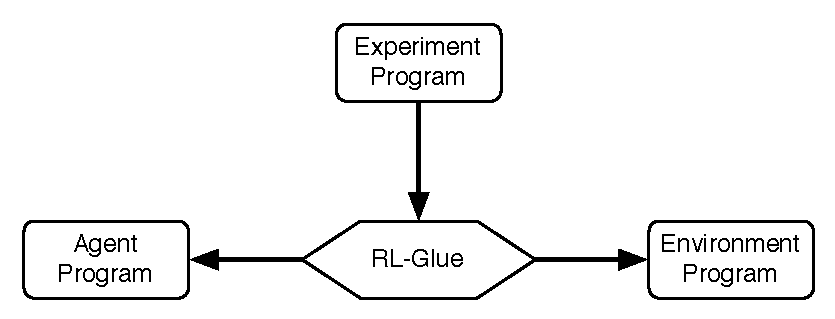
\includegraphics[width=9cm]{glue.pdf}
\vspace{-0.2cm}
\caption{\small The RL-Glue Protocol splits reinforcement learning framework into four components.  Arrows indicate function call direction.}\label{fig:RLDIA}
\end{center}
\vspace{-0.4cm}
\end{figure}

%<<<<<<< .mine
%%Brian: I agree with Shimon when he made this point about the AIM paper, we can't cite a paper that doesn't exist.  Perhaps you guys can release a tech report before this gets submitted.
%\citeauthor{whitesutton}'s RL-Glue Protocol (\citeyear{whitesutton}), illustrated in Figure \ref{fig:RLDIA}, separates the reinforcement learning framework into four main components: the agent program, environment program, experiment program and the RL-Glue interface. The agent program contains the learning algorithm and action selection mechanism. The environment program implements the dynamics of the task and generates the rewards. The experiment program controls the experiment's execution, including the sequence of agent-environment interactions and collects statistics about the agent's performance.  The RL-Glue interface mediates the communication between the agent and environment programs in response to commands from the experiment program. 
%=======
%>>>>>>> .r992

The RL-Glue Software (RL-Glue) is an implementation of \citeauthor{whiteThesis}'s RL-Glue Protocol.  RL-Glue can be used either in {\it internal} or {\it external} mode.  When using \textit{internal} mode, the agent, environment and experiment are linked into a single program, and their communication is through function calls.  Internal mode is currently an option if the agent, environment, and experiment are written exclusively in Java or C/C++.  When using  \textit{external} mode, the agent, environment and experiment are linked into separate programs.  Each program connects to the RL-Glue server program, and all communication is over TCP/IP socket connections. The external mode allows these programs to be written in any programming language that supports socket communication.  External mode is currently supported for C/C++, Java, Python, Lisp, and Matlab.

Each mode has its strengths and weaknesses. Internal mode has less overhead, so it can execute more steps per second. External mode is more flexible and portable.  The performance difference between the two modes vanishes as the agent or environment becomes complex and that computation dominates the socket overhead in terms of time per step.  The agent and environment programs are completely agnostic of their execution mode, the difference is only in how they are linked or loaded.

%This feels out of place, maybe it's better after the software intro... moving.
%Nope, still feels out of place, commenting out for now
%The RL-Glue Software is a language independent implemention of the RL-Glue Protocol  that allows agent, environment and experiment programs to be developed in different languages, and run on different computers over the internet. Please refer to the RL-Glue Software Project website for the latest code, documentation and subversion access:  {\url http://glue.rl-community.org/}

%This also felt out of place
%The current release of the RL-Glue Software includes support for Java, C/C++, Matlab, Python and Lisp. 

%UGH, I am not feelin this either.  Just feels not right here.  I will come back and try some things tomorrow
%The RL-Glue software also provides a means for sending the agent program a simple and concise message that describes the environment. The message allows the agent to, generally speaking, adapt itself to best learn about the environment.  This information can also be used to check that the agent and environment are compatible or provide the agent with prior information. A more complete description of RL-Glue's Task Specification Language can be found here: {\url http://glue.rl-community.org/Home/rl-glue/task-spec-language}.




\section{RL-Glue in Practice}
RL-Glue has provided a common interface for a number of software and hardware projects in the reinforcement learning community.  For example, there is an annual competition,\footnote{\url{http://www.rl-competition.org/}} where teams from around the world compare their learning algorithms on a variety of challenging environments.  The competition software uses an API\footnote{\url{http://code.google.com/p/rl-viz/}} that is layered on top of RL-Glue to dynamically load agent and environment programs, modify parameters at runtime and visualize interaction and performance.  All of the environments and sample agents, provided with the competition software, are added to the RL-Library,\footnote{\url{http://library.rl-community.org/}} a public, community-supported repository of RL-Glue compatible code. Additionally, the RL-Library has been designed as anarchive for top competition agents, experiment code used in publications, challenge problems and state of the art agent programs. 



The socket architecture of RL-Glue allows diverse soft and hard -ware platforms to be connected as RL-Glue environment programs.  There are ongoing projects that connect a mobile robot platform,\footnote{\url{http://www.cs.ualberta.ca/~sokolsky/critterbot/}} the keepaway soccer server, a real-time strategy game, and an Atari emulator to RL-Glue. Our socket architecture helps lower the barriers for researchers wishing to work on larger scale environments by providing a simple and familiar interface. %These environments will soon be accessible via RL-Library. 

RL-Glue has been used for teaching reinforcement learning in several university courses and to create experiments for scientific articles published in leading conferences. We maintain an updated list\footnote{\url{http://glue.rl-community.org/rl-glue-in-practice}} of all known projects that have benefited from RL-Glue.



\section{Other Reinforcement Learning Software Projects}
RL-Glue is not the first software project that aims to  standardize empirical reinforcement learning or to make agent and environment programs more accessible within our community.  However, RL-Glue is the only project that offers a standardized language-independent interface, rich actions and observations, and fine-grained control of the experiment.

Other projects, most notably: CLSquare,\footnote{\url{http://www.ni.uos.de/index.php?id=70}}  PIQLE,\footnote{\url{http://piqle.sourceforge.net/}} RL Toolbox,\footnote{\url{http://www.igi.tugraz.at/ril-toolbox/}
} JRLF,\footnote{\url{http://mykel.kochenderfer.com/jrlf/}}  and LibPG,\footnote{\url{http://code.google.com/p/libpgrl/}} offer significant value to the reinforcement learning community by offering agents and environments, intuitive visualizations, programming tools, etc.  Users should not be forced to choose between RL-Glue and these alternative projects. Our design goals makes it relatively easy to interface existing frameworks with RL-Glue.  We are eager to offer assistance in bridging these frameworks to RL-Glue, with the hope of improving access to all of these tools for all members of our community.





 
 
 
\section{RL-Glue Open Source Project}
\begin{tabular}{ l l }
  Website &  \url{http://glue.rl-community.org} \\
  License & Apache 2.0  \\
\end{tabular}
\newline
\newline
RL-Glue is more than an interface, it connects a family of community projects, with many levels of possible participation. The community is invited to submit agent, environment and experiment programs to the RL-Library. Developers can also extend the reach of RL-Glue compatibility by writing external or internal -mode interfaces for their favorite programming language.  The RL-Glue Software project also welcomes code submissions and improvements for all parts of the code base.  

% The RL-Glue Software Project has received significant contributions at many of the levels discussed above. The Lisp socket code was contributed by Gabor Balazs. Jose Antonio Martin H. developed a native windows implementation of the RL-Glue Software. The RL-Library has also received several environments submitted from previous competitions participants and paper authors.
%Webpage detailing project contributions?
%Brian: That's a good idea. Very good.

%Brian: Obviously, this is  WAY out of place.



\section{Acknowledgements}
We would like to thank all of the users, testers, and developers for their contributions to RL-Glue 3.0. Special thanks to 
Gabor Balasz,  %get the accents right
Jose Antonio Martin H.,  %get the accents right
Scott Livingston, %Middle Initial?
Marc Bellemare, 
Istvan Svita,  %get the accents right
Marc Lanctot, 
Anna Koop, 
Dan Lizotte,
Richard Sutton,
Monica Dinculescu,
Jordan Frank, and
Andrew Butcher.  Of course, we also owe a great debt to all of the talented people responsible for the historic and ongoing development of RL-Glue.\footnote{\url{http://site-with-contributions}}

% \section{History of RL-Glue}
% The RL-Glue Software project has gone through several iterations adding new features, supported languages and developers. The first release of the software, RL-Glue 1.0 in 2005, provided support for C/C++, Java and Python through a file-pipe interface. The primary contributors at the time were Adam White, Mark Lee and Richard Sutton. The next release of the software, RL-Glue 2.0 in 2007, introduced the socket communication architecture. RL-Glue 2.0 was created by White, Andrew Butcher, Lee, and Brian Tanner. The current release adds new languages (Matlab and Lisp), new example projects, platform-specific distributions, install programs, extensive documentation, and more.  The primary developer of RL-Glue 3.0 is Brian Tanner.
   



%\addcontentsline{toc}{chapter}{Bibliography}
     %add the above line to get "Bibliography" in the table of contents.
%
%\singlespacing % optional;  Bibliography is better in single spacing
               %            but you may choose different
               %            Don't use \singlespacing if your thesis
               %            is already in single spacing
%
                          % for long bibs.


\bibliographystyle{natbib}
\bibliography{jmlrTake2}



\end{document}  